\documentclass[12pt]{article}
\usepackage[utf8]{inputenc}
\usepackage{amsmath, amssymb}
\usepackage{xcolor}
\usepackage{geometry}
\usepackage{hyperref}
\usepackage{fancyhdr}
\usepackage{enumitem}
\usepackage{minted} % Code highlighting
\usepackage{booktabs} % Clean tables
\usepackage{tikz} % Optional for concept maps
\usepackage{graphicx}

\geometry{margin=1in}
\hypersetup{colorlinks=true, linkcolor=blue, urlcolor=cyan}

\pagestyle{fancy}
\fancyhf{}
\fancyhead[L]{\textbf{\TOPICTITLE}}
\fancyhead[R]{\thepage}

% -------------------------------
% Topic Metadata
% -------------------------------
\newcommand{\TOPICTITLE}{Cloud and Parallel Computing}
\title{\TOPICTITLE\\\large Study-Ready Notes}
\author{Compiled by Andrew Photinakis}
\date{\today}

\setlength{\headheight}{15pt}

\begin{document}
\maketitle
\tableofcontents
\newpage

% This LaTeX file should be saved at: parallel_computing/week06/cloud_and_parallel_computing.tex

\section{Introduction to Cloud Computing}

\subsection{Motivation for Cloud Computing}
\begin{itemize}
    \item \textbf{Business Perspective:}
          \begin{itemize}
              \item Cost reduction through shared infrastructure
              \item Scalability to meet fluctuating demand
              \item Access to enterprise-level computing resources
          \end{itemize}

    \item \textbf{Research Perspective:}
          \begin{itemize}
              \item Access to high-performance computing without capital investment
              \item Ability to process large datasets
              \item Collaborative research across institutions
          \end{itemize}
\end{itemize}

\textcolor{blue}{[Summary: Cloud computing provides scalable, cost-effective computing resources for both business and research applications, eliminating the need for significant upfront hardware investments.]}

\subsection{Definition of Cloud Computing}
\begin{itemize}
    \item Distributed systems of virtualized computers
    \item Provides services to match providers and consumers
    \item Resources are abstracted through virtualization
\end{itemize}

\section{Types of Cloud Computing}

\subsection{Deployment Models}
\begin{itemize}
    \item \textbf{Public Cloud:} Services available to general public over internet
    \item \textbf{Private Cloud:} Dedicated infrastructure for single organization
    \item \textbf{Edge Computing:} Processing at network edge near data sources
\end{itemize}

\subsection{Service Models}
\begin{itemize}
    \item \textbf{Infrastructure as a Service (IaaS):} Virtual machines, storage, networking
    \item \textbf{Platform as a Service (PaaS):} Development platforms and tools
    \item \textbf{Software as a Service (SaaS):} Applications delivered over web
\end{itemize}

\textcolor{teal}{[Concept Map: Cloud Types → Deployment (Public/Private/Edge) × Service (IaaS/PaaS/SaaS)]}

\section{Benefits of Cloud Computing}

\subsection{Service Provider Benefits}
\begin{itemize}
    \item Dynamic scaling to match customer demand
    \item Cost advantages through resource sharing
    \item On-demand service delivery
    \item Information hiding through virtualization
\end{itemize}

\subsection{Consumer Benefits}
\begin{itemize}
    \item Seemingly infinite resource pool
    \item Little additional capital expenses
    \item On-demand resource provisioning
    \item Robust to failures (no single point of failure)
    \item Cost reduction and security/privacy features
\end{itemize}

\section{Cloud Service Models}

\subsection{Everything as a Service (XaaS)}
\begin{itemize}
    \item \textbf{Infrastructure as a Service (IaaS):}
          \begin{itemize}
              \item Virtual machine instances
              \item Storage services
              \item Dynamic resource provisioning
          \end{itemize}

    \item \textbf{Platform as a Service (PaaS):}
          \begin{itemize}
              \item Development frameworks
              \item Middleware services
              \item Deployment platforms
          \end{itemize}

    \item \textbf{Software as a Service (SaaS):}
          \begin{itemize}
              \item Web-based applications
              \item No local installation required
              \item Automatic updates
          \end{itemize}
\end{itemize}

\textcolor{blue}{[Summary: Cloud services provide the illusion of unique, secure infrastructure with dynamic scaling, security, and performance guarantees through various service models.]}

\subsection{Infrastructure as a Service (IaaS)}
\begin{itemize}
    \item Access to parallel computers (virtual machines)
    \item Dynamic provisioning of computing resources
    \item Suitable for parallelizable applications:
          \begin{itemize}
              \item Weather modeling and prediction
              \item Financial analysis and risk modeling
              \item Scientific simulations
          \end{itemize}
\end{itemize}

\section{Parallel Computing in Cloud Environments}

\subsection{Cloud Processing Architecture}
\begin{itemize}
    \item Multiple processing units with many cores
    \item GPU acceleration support
    \item Efficient resource utilization through:
          \begin{itemize}
              \item Task scheduling and load balancing
              \item Performance optimization
              \item Energy consumption management
              \item Monetary cost optimization
          \end{itemize}
    \item Access to distributed cloud storage
    \item MapReduce for large-scale data processing
\end{itemize}

\subsection{Cost Models for Parallel Computing}

\subsubsection{Traditional Parallel Computing Cost}
\[
    \text{Cost} = T_p \times P
\]
Where:
\begin{itemize}
    \item $T_p$ = Execution time
    \item $P$ = Number of processors
\end{itemize}

\subsubsection{Cloud Computing Cost}
\[
    \text{Cost} = T_p \times P \times C_x
\]
Where:
\begin{itemize}
    \item $C_x$ = Service provider cost per processor (in dollars)
    \item $C_x$ may vary with time of day or week
    \item Multi-objective optimization required:
          \begin{itemize}
              \item Latency minimization
              \item Monetary cost reduction
              \item Energy consumption optimization
          \end{itemize}
\end{itemize}

\textcolor{orange}{[Mnemonic: Cloud Cost = Time × Processors × Variable Rate]}

\section{Cloud Computing Models}

\subsection{MapReduce for Large Files}
\begin{itemize}
    \item Designed for read/write operations with large files
    \item Not optimized for inter-processor communications
    \item Suitable for batch processing of large datasets
\end{itemize}

\subsection{MPI for Multi-Unit Systems}
\begin{itemize}
    \item Message Passing Interface support needed
    \item Enables communications among systems/processors
    \item Better for tightly-coupled parallel applications
\end{itemize}

\section{Elasticity in Cloud Computing}

\subsection{Definition and Importance}
\begin{itemize}
    \item Ability to meet varying computational demands
    \item Dynamic resource allocation based on workload
\end{itemize}

\subsection{Elastic Parallel Systems}
\begin{itemize}
    \item Control number of processing units at run-time
    \item Elastic controller for optimal resource utilization
    \item Number of processor units is time-dependent: $P(t)$
    \item Cost per processor may vary with time: $C_x(t)$
    \item Support for heterogeneous processing units
\end{itemize}

\textcolor{blue}{[Summary: Elasticity allows cloud systems to dynamically adjust computing resources in response to changing workloads, optimizing both performance and cost.]}

\subsection{Challenges in Elastic Parallel Computing}
\begin{itemize}
    \item Complex relationship between:
          \begin{itemize}
              \item Number and duration of computing steps
              \item Processor capacity and execution time
              \item Elastic speedup and efficiency metrics
          \end{itemize}
\end{itemize}

\section{Designing Elastic Parallel Systems}

\subsection{Key Considerations}
\begin{itemize}
    \item \textbf{Application Analysis:}
          \begin{itemize}
              \item Workload patterns of target problems
              \item Resource intensity variations
          \end{itemize}

    \item \textbf{Resource Mapping:}
          \begin{itemize}
              \item Match workload patterns to available cloud resources
              \item Cost-efficiency tradeoff analysis
          \end{itemize}

    \item \textbf{Scaling Strategies:}
          \begin{itemize}
              \item Horizontal vs. vertical scaling decisions
              \item Evaluation of elastic parallel systems
          \end{itemize}

    \item \textbf{Control Mechanisms:}
          \begin{itemize}
              \item Understanding elasticity-related opportunities
              \item Implementation of dynamic resource controllers
          \end{itemize}
\end{itemize}

\section{MapReduce Architecture}

\subsection{System Components}
\begin{itemize}
    \item \textbf{Input Data:} Large datasets divided into chunks
    \item \textbf{Map Phase:} Multiple worker nodes process data chunks
    \item \textbf{Master Node:} Coordinates overall process
    \item \textbf{Intermediary Results:} Temporary output from map phase
    \item \textbf{Reduce Phase:} Worker nodes combine intermediary results
    \item \textbf{Final Results:} Output written to file system
\end{itemize}

\begin{figure}[h]
    \centering
    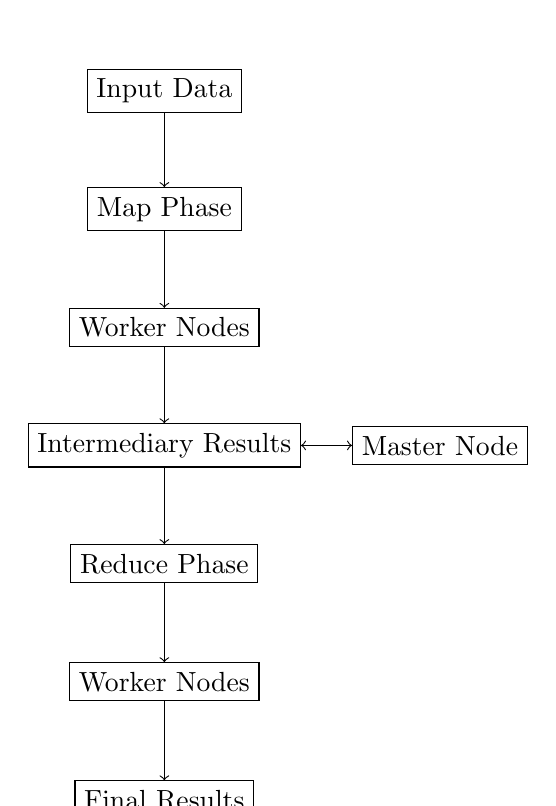
\begin{tikzpicture}[node distance=1.5cm]
        \node[draw, rectangle] (input) {Input Data};
        \node[draw, rectangle, below of=input] (map) {Map Phase};
        \node[draw, rectangle, below of=map] (workers1) {Worker Nodes};
        \node[draw, rectangle, below of=workers1] (intermediate) {Intermediary Results};
        \node[draw, rectangle, below of=intermediate] (reduce) {Reduce Phase};
        \node[draw, rectangle, below of=reduce] (workers2) {Worker Nodes};
        \node[draw, rectangle, below of=workers2] (output) {Final Results};
        \node[draw, rectangle, right of=intermediate, xshift=2cm] (master) {Master Node};

        \draw[->] (input) -- (map);
        \draw[->] (map) -- (workers1);
        \draw[->] (workers1) -- (intermediate);
        \draw[->] (intermediate) -- (reduce);
        \draw[->] (reduce) -- (workers2);
        \draw[->] (workers2) -- (output);
        \draw[<->] (master) -- (intermediate);
    \end{tikzpicture}
    \caption{MapReduce Architecture Diagram}
    \label{fig:mapreduce-arch}
\end{figure}

\subsection{MapReduce Process Flow}
\begin{enumerate}
    \item \textbf{Input Partitioning:}
          \begin{itemize}
              \item Break input data into small chunks
              \item Data typically stored in distributed file system (e.g., Google File System)
          \end{itemize}

    \item \textbf{Map Phase:}
          \begin{itemize}
              \item Initial processing on data chunks
              \item Produce intermediary key-value pairs
              \item Results buffered in distributed storage
          \end{itemize}

    \item \textbf{Reduce Phase:}
          \begin{itemize}
              \item Combine intermediary results
              \item Produce final output
              \item Results stored in output files
          \end{itemize}
\end{enumerate}

\section{MapReduce Examples and Applications}

\subsection{Common Use Cases}
\begin{table}[h]
    \centering
    \begin{tabular}{p{3cm}p{4cm}p{4cm}p{3cm}}
        \toprule
        \textbf{Function} & \textbf{Map Phase}                                       & \textbf{Intermediate Step} & \textbf{Reduce Phase}         \\
        \midrule
        Word Count        & For each word occurrence, emit $\langle$word, 1$\rangle$ & Merge/sort by key          & Count 1s for each word        \\
        \hline
        Grep              & Output lines matching pattern                            & Identity operation         & Concatenate results           \\
        \hline
        Sort              & Emit key-value pairs for sorting                         & Sort by key                & Identity operation            \\
        \hline
        Inverted Index    & Emit $\langle$word, document ID$\rangle$ pairs           & Group by word              & Produce sorted document lists \\
        \bottomrule
    \end{tabular}
    \caption{MapReduce Examples and Their Processing Steps}
    \label{tab:mapreduce-examples}
\end{table}

\textcolor{orange}{[Mnemonic: Map = Process chunks, Reduce = Combine results]}

\subsection{Main Processing Steps}
\begin{itemize}
    \item \textbf{Data Partitioning:}
          \begin{itemize}
              \item Key-value operations over different data chunks
              \item Parallelism achieved through input data division
          \end{itemize}

    \item \textbf{Intermediate Processing:}
          \begin{itemize}
              \item Compute key-value/associated value pairs
              \item Parallel computation of intermediate data
          \end{itemize}

    \item \textbf{Reduction Phase:}
          \begin{itemize}
              \item Merge and/or group pairs
              \item Separate reduction per group
              \item Parallel reduction over groups
          \end{itemize}
\end{itemize}

\section{MapReduce Advantages and Limitations}

\subsection{Positive Aspects}
\begin{itemize}
    \item \textbf{Simplicity and Ease of Use:}
          \begin{itemize}
              \item Programmer doesn't specify job distribution
              \item Number of map tasks depends on input blocks, not processors
          \end{itemize}

    \item \textbf{Flexibility:}
          \begin{itemize}
              \item Handles irregular and unstructured data
              \item Adaptable to various data formats
          \end{itemize}

    \item \textbf{Fault Tolerance:}
          \begin{itemize}
              \item Resilient to worker failures
              \item Master pings workers and reschedules if necessary
          \end{itemize}

    \item \textbf{Scalability:}
          \begin{itemize}
              \item Highly scalable across many nodes
              \item Linear scaling with data size
          \end{itemize}
\end{itemize}

\subsection{Challenges and Limitations}
\begin{itemize}
    \item \textbf{Low Efficiency:}
          \begin{itemize}
              \item Poor I/O efficiency due to disk operations
              \item Map and Reduce are blocking operations
          \end{itemize}

    \item \textbf{Synchronization Overhead:}
          \begin{itemize}
              \item No transition to next stage until current stage completes
              \item Difficult to implement pipelined operations
          \end{itemize}

    \item \textbf{High Latency:}
          \begin{itemize}
              \item Batch processing nature introduces delays
              \item Not suitable for real-time processing
          \end{itemize}
\end{itemize}

\textcolor{blue}{[Summary: MapReduce provides simple, fault-tolerant data processing but suffers from I/O inefficiency and high latency due to its batch-oriented, synchronized design.]}

\section{Advanced Example: Minimum Spanning Tree with MapReduce}

\subsection{Problem Formulation}
Given graph $G(V, E)$ where:
\begin{itemize}
    \item $V$ = set of vertices
    \item $E$ = set of edges
    \item $N$ = number of vertices
\end{itemize}

\subsection{MapReduce Algorithm Steps}
\begin{enumerate}
    \item \textbf{Random Partitioning:}
          \begin{itemize}
              \item Partition vertices into $k$ equal-sized subsets
              \item $V_1 \cup V_2 \cup V_3 \cup \dots \cup V_k = V$
              \item $V_i \cap V_j = \emptyset$ for $i \neq j$
              \item Each subset contains $N/k$ vertices
          \end{itemize}

    \item \textbf{Edge Set Definition:}
          \begin{itemize}
              \item $E_{i,j} \subseteq E$ is the set of edges induced by $V_i \cup V_j$
              \item $E_{i,j} = \{(u,v) \in E \mid u,v \in V_i \cup V_j\}$
              \item $G_{i,j} = (V_i \cup V_j, E_{i,j})$
              \item Total of $\binom{k}{2}$ subgraphs $G_{i,j}$ ("Chunks")
          \end{itemize}

    \item \textbf{Map Phase:}
          \begin{itemize}
              \item Compute unique minimum spanning forest $M_{i,j}$ for each $G_{i,j}$
          \end{itemize}

    \item \textbf{Aggregation:}
          \begin{itemize}
              \item Compute $H = (V, \bigcup_{i,j} M_{i,j})$
          \end{itemize}

    \item \textbf{Reduce Phase:}
          \begin{itemize}
              \item Compute $M$ = minimum spanning tree of $H$
          \end{itemize}
\end{enumerate}

\subsection{Mathematical Formulation}
\begin{align*}
     & \text{Partition: } V = \bigcup_{i=1}^k V_i, \quad V_i \cap V_j = \emptyset \text{ for } i \neq j                              \\
     & \text{Subgraphs: } G_{i,j} = (V_i \cup V_j, E_{i,j}), \quad \text{where } E_{i,j} = \{(u,v) \in E \mid u,v \in V_i \cup V_j\} \\
     & \text{Map: } M_{i,j} = \text{MST}(G_{i,j})                                                                                    \\
     & \text{Aggregate: } H = \left(V, \bigcup_{1 \leq i < j \leq k} M_{i,j}\right)                                                  \\
     & \text{Reduce: } M = \text{MST}(H)
\end{align*}

\textcolor{teal}{[Concept Map: MST with MapReduce → Partition → Local MSTs (Map) → Combine (Aggregate) → Global MST (Reduce)]}

\textbf{Reference:} Karloff, Howard, Siddharth Suri, and Sergei Vassilvitskii. "A model of computation for MapReduce." In Proceedings of the twenty-first annual ACM-SIAM symposium on Discrete Algorithms, pp. 938-948. Society for Industrial and Applied Mathematics, 2010.

\end{document}